\problemname{Pixelproblem}

Simon tycker att det är trevligt med bilder. Han samlar på alla sorters bilder:
vackra algoritmiskt genererade bilder, norrländska landskap och skärmdumpar av
diverse obskyra matematiska bevis, för att nämna några. Dessa är långt ifrån
alla kategorier av bilder som Simon har i sin samling.

Nu har det dock strulat till sig ordentligt. Simons hårddisk har gått sönder.
Som tur var så lyckades han rädda några av bilderna, men bara färgdatan. Han
har med andra ord \emph{inte en aning} om vilka dimensioner bilderna hade. Och
inte nog med det - det verkar dessutom som att Simon kanske inte har lyckats
återställa alla pixlar i bilderna. Det enda Simon är säker på är att minst en
pixel på sista raden i varje bild är kvar, och alla pixlar på sista raden som
är kvar är sammanhängande. Den sista raden \emph{kan} alltså ha blivit avklippt
vid någon position.

\begin{figure}[ht!]
\centering
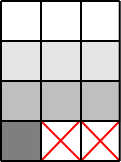
\includegraphics[width=0.2\textwidth]{example.png}
\caption{Miniatyr-exempel på hur en bild kan se ut efter Simons hårddisk-krasch. Indata
för denna bild skulle bestå av 10 pixlar i listan (två har gått förlorade), och de vita
pixlarna skulle komma först, sedan de grå, osv. Genom att titta på bildens pixlar kan
man konstatera att ursprungsbredden antagligen var 3 pixlar.}
\end{figure}

Nu behöver Simon experthjälp för att ta reda på bildernas dimensioner utifrån
färgdatan och informationen ovan. I sin desperation går Simon in på den
välkända Internet-sökmotorn Lolgee och söker på \texttt{"algoritmproffs"}.
Första träffen är förstås \emph{Programmeringsolympiaden}. Det är din uppgift
att hjälpa Simon så gott du kan.

\section*{Indata}
Varje testfall innehåller precis en bild.

Indata börjar med ett heltal $100 \leq N \leq 250\,000$ på första raden, antalet pixlar vars
färgvärden Simon lyckats återställa. Du vet alltså att bilden innehöll minst
$N$ pixlar (och kanske exakt $N$ pixlar), men du vet inte hur många pixlar som
har försvunnit på sista raden i bilden. Du vet också att ursprungsbredden för
bilden var minst $20$ pixlar, och likaså den ursprungliga höjden.

Sedan följer en rad med $3N$ heltal, en lista med RGB-värden för varje pixel.
Pixlarna ges i den ordning som de lagras i Simons dator, dvs i \emph{row-major
order} (se figur ovan). Värdena för varje pixel ges i ordningen \emph{röd,
grön, blå}. Varje värde är ett heltal mellan $0$ och $255$.

Du kan läsa mer om RGB-färgmodellen på Wikipedia: \url{http://en.wikipedia.org/wiki/RGB_color_model}

\section*{Utdata}
Du ska skriva ut ett enda heltal: bildens ursprungliga bredd.

\section*{Exempel}
Det finns ett antal exempel-bilder, mot tillhörande indata och utdata som du
kan ladda ner som en zip-fil på \url{http://progolymp.se/pixel.zip}.

"sample0x.in" innehåller bildens färgdata, som beskriven ovan (med sista raden avklippt).
"sample0x.ans" innehåller svaret, dvs bildens ursprungliga bredd.
"sample0x.png/jpg" är den ursprungliga bilden, i PNG- eller JPEG-format.

\section*{Poängsättning}
Ditt program kommer testas på 25 bilder och får 4 poäng för varje rätt svar.
